\chapter{軸対称 Poisson 方程式の数値解法}
\label{app:axisym-poisson}

第2章では、球対称 Poisson 方程式を1次元の境界値問題として解き、有限差分法の精度を検証した。
本付録では、Ryden §6.5 の軸対称系を題材として、同じ中心差分の考え方を $(R,z)$ の2次元格子へ広げる\cite{ryden2025}。
2次元 Poisson 方程式の数値解法は、本書で加えた数値計算上の発展である。
近傍点を結ぶ差分式から疎行列を構成し、境界条件を組み込んで解く手順を学ぶ。

検証には、密度とポテンシャルの解析式が分かる Miyamoto--Nagai モデルを使う。
対称軸の処理と格子点の番号付けを確認したうえで、解析解との比較、残差、格子収束試験によって結果を判断する。
本付録は第2章の発展内容であり、第3章や付録\ref{app:orbit-applications}の軌道計算の前提ではない。

\begin{learningbox}[本付録で学ぶこと]
\begin{itemize}
\item 軸対称 Poisson 方程式を、計算領域と境界条件を定めた2次元の境界値問題として設定できる。
\item 中心差分を2次元へ拡張し、対称軸での滑らかさを使って軸上の差分式を導ける。
\item 格子点と未知数番号を対応させ、既知の境界値を右辺に組み込んだ疎行列の連立一次方程式を構成できる。
\item 解析解との比較と格子収束試験から、2次元有限差分解の誤差と収束次数を評価できる。
\item 残差とポテンシャルの誤差を区別し、境界条件の近似誤差を除いて離散化誤差を検証する理由を説明できる。
\end{itemize}
\end{learningbox}

数値実験は、単独で実行できる Notebook B で行う。
本文では差分式と短い実装の対応を示し、完全なソルバーと作図は Notebook に置く。
数値計算法は幸谷第8章と§14.2.3の疎行列・2次元 Poisson 方程式の説明を参考にする\cite{kouya2021}。

\section{軸対称 Poisson 方程式と検証用モデル}
\label{sec:appB-2d-poisson-intro}

円筒座標 $(R,\phi,z)$ で軸対称性 $\partial/\partial\phi=0$ を仮定すると、Poisson 方程式は
\begin{equation}
 \boxed{\frac{\partial^2\Phi}{\partial R^2}+\frac{1}{R}\frac{\partial\Phi}{\partial R}+\frac{\partial^2\Phi}{\partial z^2}=4\pi G\rho(R,z)}
\label{eq:appB-axisym-poisson}
\end{equation}
となる。
球対称の場合と異なり、$R$ だけでなく $z$ による変化も求める必要がある。
既知の密度 $\rho(R,z)$ を右辺に与え、境界条件と合わせて未知の $\Phi(R,z)$ を決める。

\subsection{検証用の Miyamoto--Nagai モデル}

密度とポテンシャルの両方が解析的に分かれば、密度を入力として得た数値解を、ポテンシャルの解析式と比較できる。
ここでは、全質量を $M$、長さのパラメータを $a>0$、$b>0$ とする Miyamoto--Nagai モデルを使う。
\begin{equation}
 B\equiv\sqrt{z^2+b^2}
\end{equation}
とおくと、ポテンシャルは
\begin{equation}
 \Phi(R,z)=-\frac{GM}{\sqrt{R^2+(a+B)^2}}
\label{eq:appB-mn-potential}
\end{equation}
であり、対応する密度は
\begin{equation}
 \rho(R,z)=\frac{b^2M}{4\pi}\frac{aR^2+(a+3B)(a+B)^2}{B^3\left[R^2+(a+B)^2\right]^{5/2}}
\label{eq:appB-mn-density}
\end{equation}
である。
$b>0$ とすることで、対称軸と円盤面を含めて滑らかなモデルを扱う。

Notebook B の既定値は
\begin{equation}
 G=M=a=1,\qquad b=0.25
\label{eq:appB-mn-units}
\end{equation}
である。
以下では、長さの基準を $a$、ポテンシャルの基準を $GM/a$ として結果を示す。
図\ref{fig:appB-mn-density}に、この設定での密度分布を示す。

\begin{figure}[!htbp]
\centering
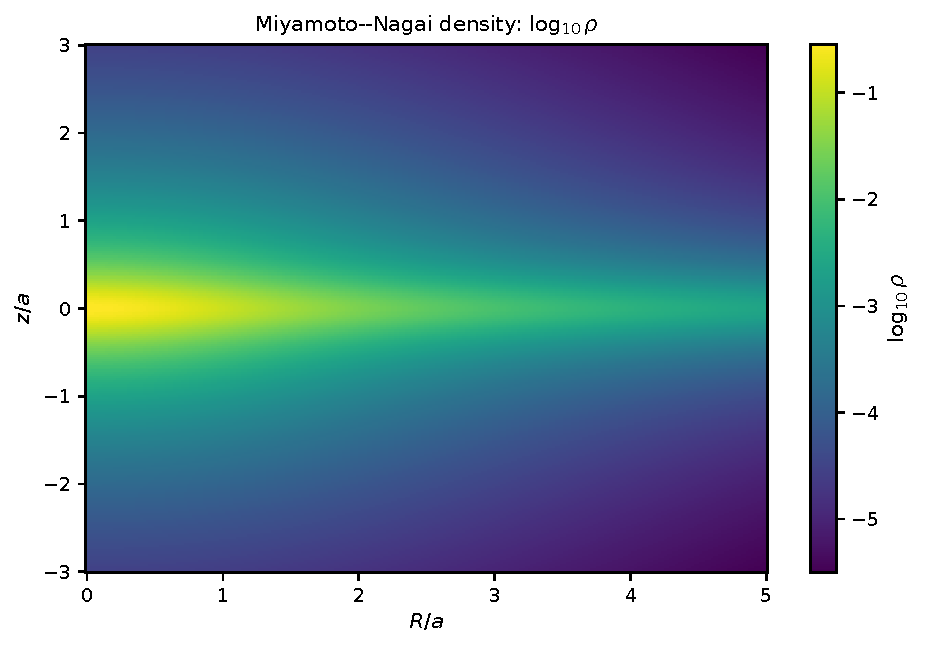
\includegraphics[width=0.64\linewidth]{appB_mn_density.pdf}
\caption{検証用の Miyamoto--Nagai モデルの密度分布。式\eqref{eq:appB-mn-units}の設定で $\log_{10}\rho$ を表示した。密度は $R$ と $z$ の両方に依存する。この図の描画用格子と、Poisson 方程式を解く格子は別に用意する。}
\label{fig:appB-mn-density}
\end{figure}

\section{2次元有限差分}
\label{sec:appB-fdm}

計算領域を $0\le R\le R_{\max}$、$-Z_{\max}\le z\le Z_{\max}$ とする。
$R$ 方向を $N_R$ 区間、$z$ 方向を $N_Z$ 区間に分け、
\begin{equation}
 \Delta R=\frac{R_{\max}}{N_R},\qquad \Delta z=\frac{2Z_{\max}}{N_Z}
\label{eq:appB-grid-spacing}
\end{equation}
とおく。両端を含む格子点は
\begin{equation}
 R_i=i\Delta R\quad(i=0,\ldots,N_R),\qquad z_j=-Z_{\max}+j\Delta z\quad(j=0,\ldots,N_Z)
\label{eq:appB-grid}
\end{equation}
である。
$N_R,N_Z$ は格子点数ではなく区間数であり、全格子点数は $(N_R+1)(N_Z+1)$ となる。
格子点上の関数値を $\Phi_{i,j}=\Phi(R_i,z_j)$ と書く。

第2章の3点ステンシル（定義2.2）を各方向へ適用する。
$R_i>0$ の内部点では、中心点と上下左右の4点を使う5点ステンシルになる（図\ref{fig:appB-stencil}）。

\subsection{$R_i>0$ の内部点}

第2章で導いた中心差分を $R$ 方向と $z$ 方向に用いると、
\begin{align}
 \left.\frac{\partial^2\Phi}{\partial R^2}\right|_{i,j}&=\frac{\Phi_{i+1,j}-2\Phi_{i,j}+\Phi_{i-1,j}}{(\Delta R)^2}+O((\Delta R)^2),\label{eq:appB-drr}\\
 \left.\frac{\partial\Phi}{\partial R}\right|_{i,j}&=\frac{\Phi_{i+1,j}-\Phi_{i-1,j}}{2\Delta R}+O((\Delta R)^2),\label{eq:appB-dr}\\
 \left.\frac{\partial^2\Phi}{\partial z^2}\right|_{i,j}&=\frac{\Phi_{i,j+1}-2\Phi_{i,j}+\Phi_{i,j-1}}{(\Delta z)^2}+O((\Delta z)^2)\label{eq:appB-dzz}
\end{align}
である。
式\eqref{eq:appB-axisym-poisson}へ代入し、打ち切り誤差を除くと、解くべき差分方程式は
\begin{equation}
 c_-\Phi_{i-1,j}+c_0\Phi_{i,j}+c_+\Phi_{i+1,j}+c_z\Phi_{i,j-1}+c_z\Phi_{i,j+1}=4\pi G\rho_{i,j}
\label{eq:appB-five-point-row}
\end{equation}
となる。以下の差分方程式で求める $\Phi_{i,j}$ は、連続なポテンシャルの数値近似である。
各点に掛かる係数をまとめると、
\begin{align}
 c_-&=\frac{1}{(\Delta R)^2}-\frac{1}{2R_i\Delta R},\label{eq:appB-cm}\\
 c_+&=\frac{1}{(\Delta R)^2}+\frac{1}{2R_i\Delta R},\label{eq:appB-cp}\\
 c_z&=\frac{1}{(\Delta z)^2},\label{eq:appB-cz}\\
 c_0&=-\frac{2}{(\Delta R)^2}-\frac{2}{(\Delta z)^2}\label{eq:appB-c0}
\end{align}
である。
動径方向では $(1/R)\partial\Phi/\partial R$ の項があるため、内側と外側の係数 $c_-,c_+$ は異なる。

\begin{figure}[!htbp]
\centering
\begin{tikzpicture}[scale=1.1]
  \foreach \x in {-1,0,1}{
    \foreach \y in {-1,0,1}{
      \fill[gray!35] (\x,\y) circle (1.4pt);
    }
  }
  \fill[navy] (0,0) circle (2.3pt);
  \fill[cyan] (1,0) circle (2.3pt);
  \fill[cyan] (-1,0) circle (2.3pt);
  \fill[cyan] (0,1) circle (2.3pt);
  \fill[cyan] (0,-1) circle (2.3pt);
  \draw[->,>=Latex] (-1.5,-1.45)--(1.55,-1.45) node[right] {$R$};
  \draw[->,>=Latex] (-1.5,-1.45)--(-1.5,1.55) node[above] {$z$};
  \node[below right] at (0,0) {$(i,j)$};
  \node[right] at (1,0) {$(i+1,j)$};
  \node[left] at (-1,0) {$(i-1,j)$};
  \node[above] at (0,1) {$(i,j+1)$};
  \node[below] at (0,-1) {$(i,j-1)$};
\end{tikzpicture}
\caption{内部格子点の5点ステンシル。差分方程式は中心点と上下左右の近傍点だけを結合する。}
\label{fig:appB-stencil}
\end{figure}

Listing B.1 では、まず $z$ 方向の中心係数を設定し、$R$ 方向の寄与を加える。
\texttt{cm}, \texttt{cp}, \texttt{cz}, \texttt{center} が、それぞれ $c_-,c_+,c_z,c_0$ に対応する。

\begin{listingbox}{B.1　内部点の差分係数}
\begin{Verbatim}[fontsize=\small]
cz = 1.0 / dz**2
center = -2.0 / dz**2
cp = 1.0 / dR**2 + 1.0 / (2.0 * Ri * dR)
cm = 1.0 / dR**2 - 1.0 / (2.0 * Ri * dR)
center += -2.0 / dR**2
\end{Verbatim}
\end{listingbox}

\subsection{対称軸 $R=0$ の処理}

式\eqref{eq:appB-axisym-poisson}の $(1/R)\partial\Phi/\partial R$ を、そのまま $R=0$ で計算することはできない。
軸上でも滑らかな軸対称ポテンシャルでは
\begin{equation}
 \left.\frac{\partial\Phi}{\partial R}\right|_{R=0}=0
\label{eq:appB-axis-symmetry}
\end{equation}
なので、この項は $0/0$ の形になる。軸へ近づく極限を先に求め、有限な式に置き換える。

$z$ を固定し、対称軸を横切る直線上に符号付き座標 $\ell$ を取ると、$R=|\ell|$ である。
軸対称性によって $\ell$ と $-\ell$ の値は等しい。
第2章§\ref{sec:ch2-boundaries}と同じく、滑らかな関数の Taylor 展開には偶数次の項だけが残るため、
\begin{equation}
 \Phi(R,z)=\Phi(0,z)+\frac{1}{2}\Phi_{RR}(0,z)R^2+O(R^4)
\label{eq:appB-axis-expansion}
\end{equation}
と書ける。ここで $\Phi_{RR}$ は $R$ による二階微分である。
$R$ で微分して $R$ で割ると、
\begin{equation}
 \frac{1}{R}\frac{\partial\Phi}{\partial R}=\Phi_{RR}(0,z)+O(R^2)
\end{equation}
なので、動径方向の二つの項を合わせた極限は
\begin{equation}
 \left[\frac{\partial^2\Phi}{\partial R^2}+\frac{1}{R}\frac{\partial\Phi}{\partial R}\right]_{R=0}=2\Phi_{RR}(0,z)
\label{eq:appB-axis-limit}
\end{equation}
となる。

さらに、対称性を用いて仮想点を $\Phi_{-1,j}=\Phi_{1,j}$ とすれば、
\begin{equation}
 \Phi_{RR}(0,z_j)=\frac{\Phi_{1,j}-2\Phi_{0,j}+\Phi_{-1,j}}{(\Delta R)^2}+O((\Delta R)^2)=\frac{2(\Phi_{1,j}-\Phi_{0,j})}{(\Delta R)^2}+O((\Delta R)^2)
\end{equation}
である。したがって、軸上で動径方向の演算子全体を近似する式は
\begin{equation}
 \boxed{2\Phi_{RR}(0,z_j)\simeq\frac{4(\Phi_{1,j}-\Phi_{0,j})}{(\Delta R)^2}}
\label{eq:appB-axis-fd}
\end{equation}
となる。この差分も、軸上での滑らかさのもとで2次精度である。
$z$ 方向の中心差分を加えた軸上の差分方程式は
\begin{align}
 \left[-\frac{4}{(\Delta R)^2}-\frac{2}{(\Delta z)^2}\right]\Phi_{0,j}+\frac{4}{(\Delta R)^2}\Phi_{1,j}\notag\\
 {}+c_z\Phi_{0,j-1}+c_z\Phi_{0,j+1}=4\pi G\rho_{0,j}
\label{eq:appB-axis-row}
\end{align}
である。

Listing B.2 は、Listing B.1 の動径方向の係数を軸上のものに置き換えたコードである。
\texttt{center} は、ここでも $z$ 方向の寄与から初期化する。
仮想点は対称性によって消去したので、負の $R$ の配列は作らない。

\begin{listingbox}{B.2　対称軸 $R=0$ の差分係数}
\begin{Verbatim}[fontsize=\small]
cz = 1.0 / dz**2
center = -2.0 / dz**2
cp = 4.0 / dR**2
center += -4.0 / dR**2
\end{Verbatim}
\end{listingbox}

\begin{cautionblock}{$1/R$ をそのまま評価しない}
ここでの $0/0$ は、滑らかなポテンシャルを円筒座標で表したことによる見かけの特異点である。
$R$ を小さな正数に置き換えるのではなく、対称軸近傍の展開から得た式\eqref{eq:appB-axis-fd}を使う。
軸対称性だけでなく、軸上で滑らかであるという仮定も必要である。
\end{cautionblock}

\section{2次元格子での連立一次方程式の組み立て}
\label{sec:appB-flatten}

第2章と同じく、差分式を連立一次方程式
\begin{equation}
 A\boldsymbol{\Phi}=\boldsymbol{b}
\label{eq:appB-linear-system}
\end{equation}
にまとめる。
ただし、2次元配列のままでは行列の列番号に対応しないため、未知格子点 $(i,j)$ に1次元の番号を付ける。
右辺ベクトル $\boldsymbol{b}$ は、密度の項と既知の境界値から作る。モデルの長さ $b$ とは別の量である。

\subsection{既知の境界と未知格子点}

$R=R_{\max}$ と $z=\pm Z_{\max}$ には、式\eqref{eq:appB-mn-potential}の解析値を与える。
この3辺の値は未知数に含めない。一方、対称軸 $R=0$ のポテンシャル値は既知ではなく、式\eqref{eq:appB-axis-row}で解く未知数に含める。
したがって、未知格子点の添字は
\begin{equation*}
 i=0,\ldots,N_R-1,\qquad j=1,\ldots,N_Z-1
\end{equation*}
である。
$z$ 方向の未知点数を
\begin{equation}
 n_z=N_Z-1
\end{equation}
とし、各 $i$ について $j$ の小さい順に並べると、
\begin{equation}
 \boxed{p=i\,n_z+(j-1)}
\label{eq:appB-index-map}
\end{equation}
で1次元番号へ写せる。
$p$ は0から $N_Rn_z-1$ までの番号であり、$\boldsymbol{\Phi}$ の第 $p$ 成分が $\Phi_{i,j}$ に対応する。
$j=0$ は境界点なので、最初の未知点 $j=1$ がオフセット0になる。

\begin{listingbox}{B.3　2次元格子の1次元番号付け}
\begin{Verbatim}[fontsize=\small]
nZ_u = NZ - 1

def idx(i, j):
    return i * nZ_u + (j - 1)
\end{Verbatim}
\end{listingbox}

Notebook B では、完全なソルバーの前に16個の未知点の番号表を表示する。
これは図\ref{fig:appB-sparse-pattern}と同じ $N_R=4$, $N_Z=5$ の例である。
逆の対応は $p$ を $n_z$ で割った商と余りから求められる。短い実装確認も同じセルの前に置いている。

\subsection{非零係数の記録と境界値の移項}

\begin{definitionbox}{定義 B.1　疎行列}
要素の大部分が0である行列を\textbf{疎行列（sparse matrix）}と呼ぶ。
有限差分法では各格子点が近傍点だけと結合するため、係数行列は典型的に疎行列になる。
\end{definitionbox}

5点ステンシルでは、一つの行に入る非零係数は高々5個である。
そこで、0も含めた全要素ではなく、非零要素の行番号・列番号・値だけを記録する。
Notebook の \texttt{rows[k]}, \texttt{cols[k]}, \texttt{data[k]} が、その三つ組に対応する。

格子点 $(i,j)$ の差分方程式を行番号 $p=\texttt{idx(i,j)}$ に割り当てる。
例えば、外側の近傍点 $(i+1,j)$ が未知点なら、その係数 $c_+$ を列番号 $q=\texttt{idx(i+1,j)}$ に入れる。
一方、$i=N_R-1$ なら近傍点は既知の外側境界なので、行列の列を作らず、
\begin{equation}
 b_p=4\pi G\rho_{i,j}-c_+\Phi_{N_R,j}^{\rm exact}
\label{eq:appB-boundary-rhs}
\end{equation}
のように右辺へ移項する。$z$ 方向にも既知の境界点があれば、その寄与も同じ符号で差し引く。

Listing B.4 は、$R_i>0$ の点における外側近傍の処理である。
\texttt{rhs[p]} は密度の項 $4\pi G\rho_{i,j}$ で初期化しておき、既知の境界値の寄与を順に差し引く。

\begin{listingbox}{B.4　未知の近傍点と既知の境界点の扱い}
\begin{Verbatim}[fontsize=\small]
if i + 1 == NR:
    rhs[p] -= cp * phi_mn(R[NR], z[j], G, M, a, b)
else:
    rows.append(p)
    cols.append(idx(i + 1, j))
    data.append(cp)
\end{Verbatim}
\end{listingbox}

同様の操作を各近傍点について行い、中心点の係数を \texttt{rows} と \texttt{cols} がともに $p$ の要素として加える。
集めた三つ組から CSR 形式の疎行列を作り、\texttt{spsolve} に行列と右辺を渡す（Listing B.5）。
CSR は非零要素を行ごとにまとめて保持する形式であり、ここでは SciPy の関数に変換を任せる\cite{kouya2021}。

\begin{listingbox}{B.5　疎行列の構成と求解}
\begin{Verbatim}[fontsize=\small]
shape = (n_unknown, n_unknown)
A = sparse.csr_matrix((data, (rows, cols)), shape=shape)
sol = spsolve(A, rhs)
\end{Verbatim}
\end{listingbox}

\texttt{sol} は1次元の解ベクトルである。
既知の境界値を2次元配列 \texttt{Phi} に設定し、未知点へ \texttt{Phi[i, j] = sol[idx(i, j)]} を代入すれば、格子全体のポテンシャルに戻せる。
疎行列の直接法における消去と代入、および消去中に非零要素が増えるフィルインについては、付録\ref{app:linear-systems}を参照する。

\medskip
\noindent\textbf{計算手順｜軸対称2次元 Poisson 方程式を解く}
\par\smallskip
\begin{enumerate}[itemsep=0em,topsep=0.1em]
\item 格子、密度、既知の境界値を用意する。
\item 未知格子点 $(i,j)$ を1次元番号 $p$ に対応させる。
\item 内部点と対称軸の差分式を使い分け、未知点の係数を記録する。
\item 既知の境界値に掛かる項は右辺へ移項する。
\item 記録した非零要素から疎行列を作り、連立一次方程式を解く。
\item 解ベクトルを2次元配列に戻し、既知の境界値と合わせる。
\end{enumerate}

\begin{cautionblock}{解析的な境界値を使う理由}
本付録では、有限の計算領域の3辺に解析値を与え、境界条件の近似誤差を除く。
領域の外にも密度は分布しており、外側の質量を捨てたモデルを解くわけではない。
解析的な境界値には、その寄与も含まれている。
これにより、解析解との差から差分による誤差を調べられる。ただし、丸め誤差や連立一次方程式の求解に伴う誤差までなくなるわけではない。
\end{cautionblock}

\section{疎行列の大きさと構造}
\label{sec:appB-sparse}

Notebook B の最初の数値解は、
\begin{equation}
 N_R=40,\qquad N_Z=64,\qquad R_{\max}=5a,\qquad Z_{\max}=4a
\label{eq:appB-main-grid}
\end{equation}
で求める。
このとき $\Delta R=\Delta z=0.125a$ である。
未知数の個数は、対称軸を含む $N_R$ 個の動径点と、上下端を除いた $N_Z-1$ 個の鉛直点の積
\begin{equation}
 N_{\rm unknown}=N_R(N_Z-1)=\appBNUnknown
\label{eq:appB-nunknown}
\end{equation}
となる。
密行列なら $N_{\rm unknown}^2=\appBNUnknown^2$ 個の要素を保存するが、実際の非零要素数は
\begin{equation}
 N_{\rm nz}=\appBNNZ
\end{equation}
であり、非零要素率は
\begin{equation}
 \frac{N_{\rm nz}}{N_{\rm unknown}^2}=\appBMatrixDensity
\label{eq:appB-matrix-density}
\end{equation}
にすぎない。Notebook では、この個数を疎行列の \texttt{nnz} から直接確認する。

図\ref{fig:appB-sparse-pattern}では、非零要素の位置を読み取るために小さい格子を使う。
式\eqref{eq:appB-index-map}から、$z$ 方向の近傍点の番号は $p\pm1$、$R$ 方向は $p\pm n_z$ となる。
例えば $(i,j)=(1,2)$ は $p=5$ に対応し、近傍点を含む列番号は $1,4,5,6,9$ である。
ただし、これらは近傍点が未知点の場合の対応であり、既知の境界点は列に含めない。
小さい行列も、数値解に使うものと同じソルバーから生成している。

\begin{figure}[!htbp]
\centering
\begin{minipage}[t]{0.48\linewidth}
 \centering
 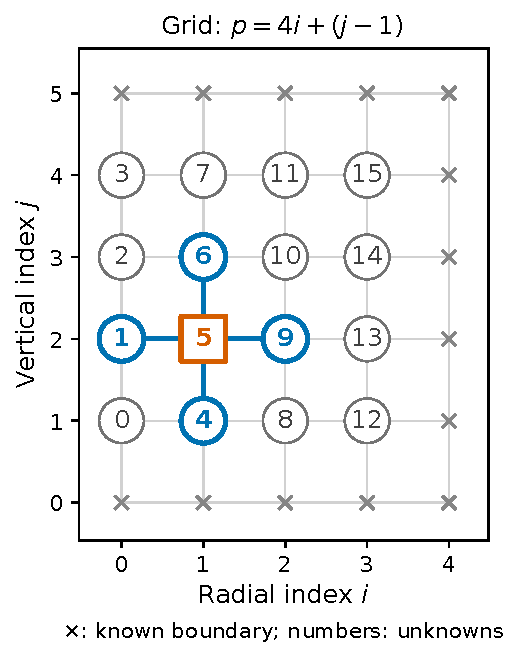
\includegraphics[height=80mm]{appB_grid_numbering.pdf}\\[-1mm]
 {\small (a) Grid numbering}
\end{minipage}\hfill
\begin{minipage}[t]{0.48\linewidth}
 \centering
 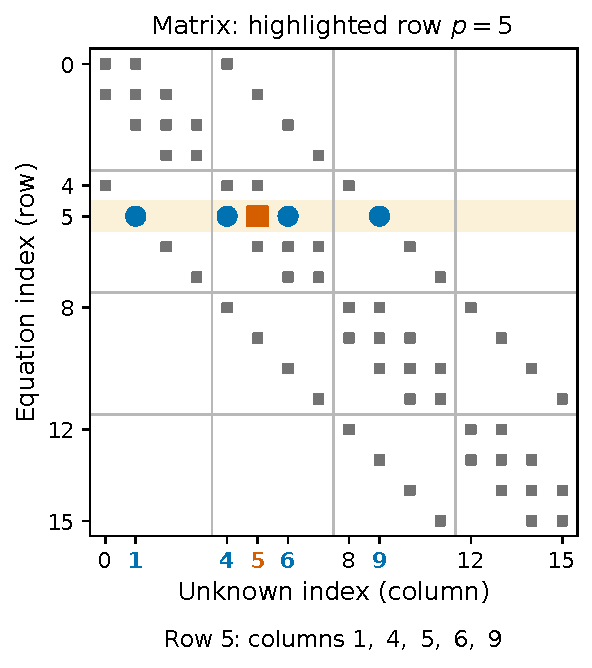
\includegraphics[height=80mm]{appB_sparse_pattern.pdf}\\[-1mm]
 {\small (b) Nonzero matrix entries}
\end{minipage}
\caption{小さい格子と疎行列の対応。説明用に $N_R=4$, $N_Z=5$（$n_z=4$、未知数16個）とした。左図の数字は未知数番号 $p$、$\times$ は既知の境界点である。赤い四角で示す $(i,j)=(1,2)$ は $p=5$ に対応し、青い丸の近傍点を含めた5点は、右図の行番号5（0始まり）の列番号 $1,4,5,6,9$ に対応する。右図の空白は零要素、灰色はその他の非零要素である。}
\label{fig:appB-sparse-pattern}
\end{figure}

番号が隣り合っていても、格子上で隣り合うとは限らない。
例えば、この図の $p=3$ と $p=4$ は動径点の切り替わりに当たり、$z$ 方向の近傍点ではない。
係数を入れる前に $(i,j)$ の範囲で境界を判定するのは、このような誤った結合を避けるためでもある。

\begin{cautionblock}{行列の記憶量と求解の計算量を分ける}
密行列の要素数は未知数の2乗で増えるが、ここで組み立てる疎行列の非零要素数は未知数にほぼ比例する。
ただし、これだけで求解の計算時間も比例すると結論することはできない。
疎行列の直接法ではフィルインも生じるため、分解中の記憶量と計算量は元の非零要素数だけでは決まらない。
\end{cautionblock}

\begin{topicblock}{シミュレーション天文学で使う重力計算法}
本付録では、Poisson 方程式を有限差分で離散化し、疎行列の連立一次方程式を解いた。
これは境界値問題の設定から数値解の検証までを学ぶための一例であり、すべての重力計算で同じ手順を使うわけではない。

\begin{itemize}
\item \textbf{滑らかな固定重力場：}
複雑な質量分布の重力場には、角度依存性を球面調和関数で表す\textbf{多重極展開（multipole expansion）}や、
密度とポテンシャルを対応する基底関数の和で表す\textbf{基底関数展開法（basis-function expansion）}などを使える。
あらかじめ構成した展開式や補間関数を微分すれば、任意の位置で加速度を評価できる。
固定場での軌道積分中に、空間上の Poisson 方程式を解き直す必要はない。
多重極展開は、第2章で紹介した遠方の境界値だけでなく、質量分布の内部の重力場を表すことにも用いられる。

\item \textbf{格子上の自己重力計算：}
一様格子では、\textbf{高速 Fourier 変換（fast Fourier transform; FFT）}を利用して
Poisson 方程式を解く方法があり、周期境界条件と組み合わせやすい。
粗い格子と細かい格子を組み合わせて離散方程式を解く\textbf{多重格子法（multigrid method）}は、
適合格子細分化法（adaptive mesh refinement; AMR）を用いる計算でも利用される。
有限差分法は方程式の\textbf{離散化}、多重格子法は離散方程式の\textbf{求解}の方法であり、
両者は組み合わせて使える。FFT も有限差分法と対立するものではなく、
有限差分で得た離散方程式を解くために利用する場合がある。

\item \textbf{粒子分布からの重力計算：}
\textbf{ツリー法（tree method）}では、遠方の粒子群からの重力を、多重極展開を使ってまとめて近似する。
\textbf{PM 法（particle-mesh method）}では、粒子の質量を格子へ割り当て、
格子上でポテンシャルと加速度を求め、加速度を粒子位置へ補間する。
格子上のポテンシャルを差分して加速度を求める実装もあり、PM 法も有限差分法と排他的な方法ではない。
重力を長距離成分と短距離成分に分け、前者を PM 法、後者をツリー法で計算する TreePM 法もある。
\end{itemize}

以上は用途に沿った例であり、排他的な分類ではない。基底関数展開を自己重力系の時間発展に用いることもできる。
研究では質量分布、境界条件、必要な空間分解能、計算規模に応じて方法を選ぶ。
方法が変わっても、参照解との比較や、格子幅・展開の項数などの近似の細かさを変えた検証は必要である。
詳しくは Binney \& Tremaine（2008）の§2.4・§2.8・§2.9\cite{bt2008}、松本ほか\cite{matsumoto}、富阪ほか編\cite{tomisaka2007}を参照すること。
\end{topicblock}

\section{数値解と誤差}
\label{sec:appB-poisson-results}

Notebook B の \texttt{solve\_mn\_poisson} は、ここまでの格子作成、係数行列と右辺の構成、求解、2次元配列への復元を一つにまとめた関数である。
同じ格子点で数値解と解析解を評価し、ポテンシャルの誤差と離散方程式の残差を別々に求める。

\begin{notebookblock}{B｜2次元 Poisson 方程式の数値解}
式\eqref{eq:appB-main-grid}の領域と区間数で解く。
\texttt{Phi\_num[i,j]} に合わせ、\texttt{meshgrid} の \texttt{indexing="ij"} によって解析解の配列も第1軸を $R$、第2軸を $z$ にする。

{\sffamily\small\color{graytext}対応セル（計算部分）}
\begin{Verbatim}[fontsize=\small,xleftmargin=2mm,frame=single,framesep=1.8mm,framerule=0.35pt,rulecolor=\color{listingframe},fillcolor=\color{listingbg}]
# 計算領域と各方向の区間数を指定する
NR, NZ = 40, 64
Rmax = 5.0 * amn
Zmax = 4.0 * amn
Rmn, zmn, Phi_num, A_mn, rhs_mn, sol_mn = solve_mn_poisson(
    NR=NR, NZ=NZ, Rmax=Rmax, Zmax=Zmax, G=G, M=Mmn, a=amn, b=bmn)

# 数値解と同じ格子上で解析ポテンシャルを評価する
RRmn, ZZmn = np.meshgrid(Rmn, zmn, indexing="ij")
Phi_exact_mn = phi_mn(RRmn, ZZmn, G, Mmn, amn, bmn)

# 解の誤差と、離散方程式の残差を別々に測る
err_phi = np.max(np.abs(Phi_num - Phi_exact_mn)) / (G * Mmn / amn)
residual = A_mn @ sol_mn - rhs_mn
residual_max = np.max(np.abs(residual))
\end{Verbatim}
\end{notebookblock}

ここで用いる誤差は、全格子点での絶対誤差の最大値を、一定の基準量 $GM/a$ で割った
\begin{equation}
 \epsilon_\Phi=\frac{\max_{i,j}|\Phi_{{\rm num},i,j}-\Phi_{{\rm exact},i,j}|}{GM/a}=\appBPhiError
\label{eq:appB-poisson-error}
\end{equation}
である。各点の $|\Phi_{\rm exact}|$ で割った相対誤差ではない。
境界には解析値を設定しているため、境界点での差は0になる。
数値ポテンシャルを図\ref{fig:appB-mn-potential}、符号付きの誤差を図\ref{fig:appB-mn-error}に示す。

\begin{figure}[!htbp]
\centering
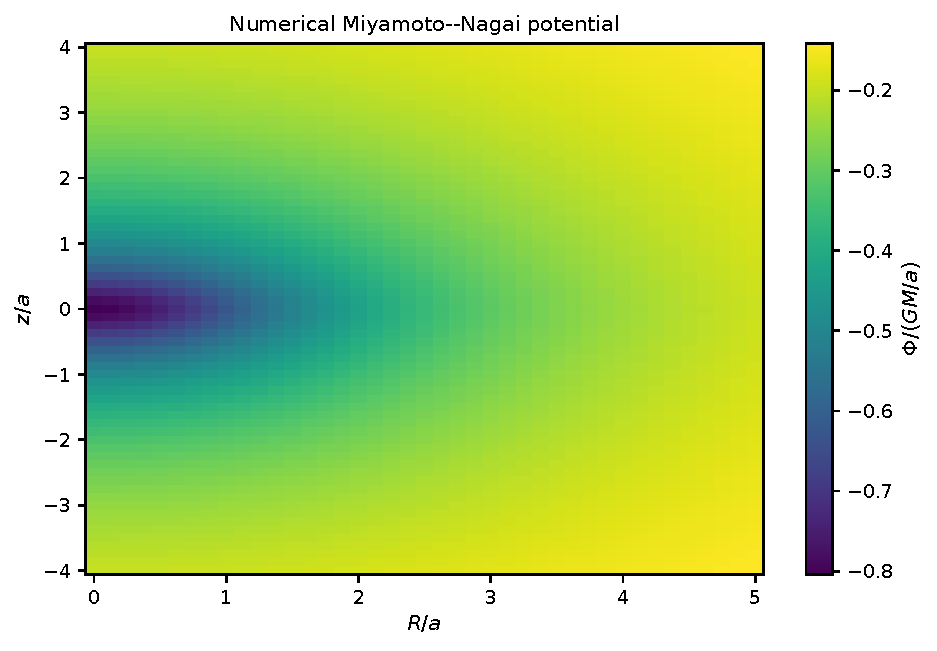
\includegraphics[width=0.64\linewidth]{appB_mn_potential.pdf}
\caption{有限差分法で求めた Miyamoto--Nagai ポテンシャル。$N_R=40$, $N_Z=64$ とし、$R=R_{\max}$ と $z=\pm Z_{\max}$ には解析値を与えた。対称軸の値は差分方程式を解いて求めている。}
\label{fig:appB-mn-potential}
\end{figure}

\begin{figure}[!htbp]
\centering
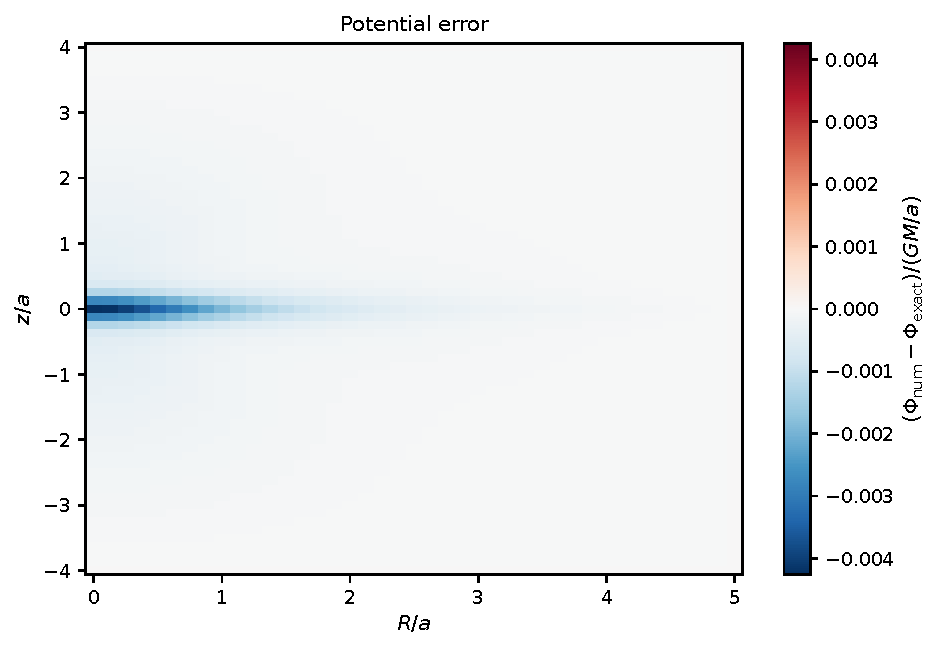
\includegraphics[width=0.64\linewidth]{appB_mn_error.pdf}
\caption{同じ格子上の数値解と解析解の差を $GM/a$ で規格化したもの。符号付き誤差を、0を中心とする対称なカラースケールで表示している。境界点での差は0である。}
\label{fig:appB-mn-error}
\end{figure}

一方、未知点の解ベクトルについて計算した最大残差は
\begin{equation}
 \max_p|(A\boldsymbol{\Phi}-\boldsymbol{b})_p|=\appBResidual
\label{eq:appB-residual}
\end{equation}
である。
これは、上で定義した差分係数を使い、$G=M=a=1$ で計算した値である。
残差は離散方程式の左右のずれであり、ポテンシャルの誤差とは単位も異なる。
方程式全体を定数倍すれば残差も定数倍されるため、異なる規格化の残差をそのまま比較しない。

\begin{cautionblock}{残差が小さくても離散化誤差は残る}
第2章の残差の定義と同じく、ここで小さい残差が示すのは、数値解が組み立てた連立一次方程式をよく満たすことである。
その方程式は連続な Poisson 方程式そのものではないため、解析解との差は残る。
ポテンシャルの精度は、式\eqref{eq:appB-poisson-error}と格子収束試験で別に確認する。
\end{cautionblock}

\section{2次元 Poisson 方程式の格子収束}
\label{sec:appB-poisson-convergence}

一つの格子で解と残差を確認した後は、領域・境界条件・モデルを固定して格子を細かくする。
内部点と対称軸で使った差分は、滑らかな解に対して各方向で2次精度である。
二つの格子幅を一定の比率で小さくすれば、離散化誤差が支配する十分細かい格子で
\begin{equation}
 \epsilon_\Phi\propto h^2,\qquad h\equiv\max(\Delta R,\Delta z)
\label{eq:appB-poisson-conv-expected}
\end{equation}
が期待される。
ただし、第2章で述べたように、差分公式の打ち切り誤差の次数だけで数値解全体の収束が保証されるわけではない。
ここでも、境界を含むソルバー全体の結果から次数を測定する。

\medskip
\noindent\textbf{検証手順｜2次元格子の収束試験}
\par\smallskip
\begin{enumerate}[itemsep=0em,topsep=0.1em]
\item $R_{\max}=5a$, $Z_{\max}=4a$、モデルのパラメータ、解析的な境界条件を固定する。
\item $N_R$ と $N_Z$ を同じ比率で増やし、両方向の格子幅を小さくする。
\item 各格子の数値解を同じ格子上の解析解と比較し、$\epsilon_\Phi$ を計算する。
\item 両対数表示の傾きから収束次数を測定し、期待する2次収束と比較する。
\end{enumerate}

Notebook B では $(N_R,N_Z)=(40,64),(60,96),(80,128),(100,160)$ とする。
この組では常に $\Delta R=\Delta z$ であり、$h/a$ は $0.125,0.08333\ldots,0.0625,0.05$ となる。
$R$ 方向だけを細かくして $\Delta z$ を固定する比較とは異なる。

\begin{notebookblock}{B｜2次元 Poisson 方程式の格子収束}
各格子で得た $\epsilon_\Phi$ と $h$ を配列に保存する。
\texttt{polyfit} では、この4格子の両対数データに直線を当てはめ、その傾きを収束次数とする。

{\sffamily\small\color{graytext}対応セル（計算部分）}
\begin{Verbatim}[fontsize=\small,xleftmargin=2mm,frame=single,framesep=1.8mm,framerule=0.35pt,rulecolor=\color{listingframe},fillcolor=\color{listingbg}]
# 領域とモデルを固定し、両方向の区間数を同じ比率で増やす
grid_list = [(40, 64), (60, 96), (80, 128), (100, 160)]
h_list = []
err_list = []

for NR_i, NZ_i in grid_list:
    R_i, z_i, Phi_i, _, _, _ = solve_mn_poisson(
        NR=NR_i, NZ=NZ_i, Rmax=Rmax, Zmax=Zmax,
        G=G, M=Mmn, a=amn, b=bmn)

    # 同じ格子上の解析解から、規格化した最大絶対誤差を測る
    RR_i, ZZ_i = np.meshgrid(R_i, z_i, indexing="ij")
    Phi_ex_i = phi_mn(RR_i, ZZ_i, G, Mmn, amn, bmn)
    h_i = max(R_i[1] - R_i[0], z_i[1] - z_i[0])
    err_i = np.max(np.abs(Phi_i - Phi_ex_i)) / (G * Mmn / amn)
    h_list.append(h_i)
    err_list.append(err_i)

h_list = np.array(h_list)
err_list = np.array(err_list)

# epsilon_Phi が h^p に比例する範囲では、両対数の傾きが p
order_2d = np.polyfit(np.log(h_list), np.log(err_list), 1)[0]
\end{Verbatim}
\end{notebookblock}

この4格子から得られる次数は
\begin{equation}
 p=\appBOrderTwoD
\label{eq:appB-poisson-conv-measured}
\end{equation}
であり、図\ref{fig:appB-poisson-convergence}のように誤差はほぼ2次で減少する。
これは、ここで用いた滑らかなモデル、解析的な境界条件、格子幅の範囲に対する実測値である。
別の密度分布や境界条件へ変更する場合も、同じ検証を繰り返す必要がある。

\begin{figure}[!htbp]
\centering
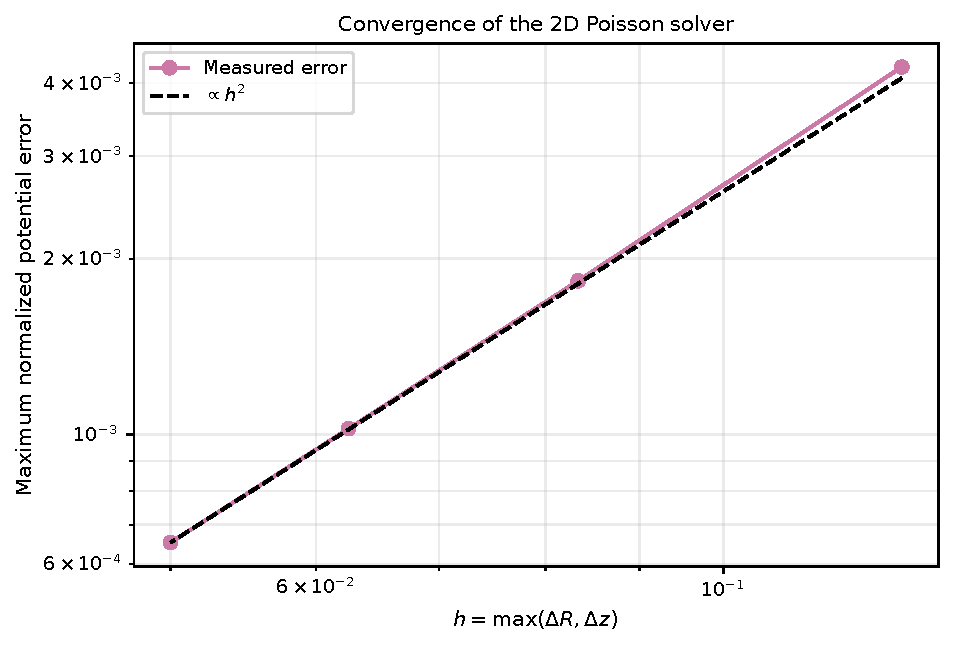
\includegraphics[width=0.64\linewidth]{appB_poisson2d_convergence.pdf}
\caption{領域と境界条件を固定した2次元 Poisson 方程式の格子収束。実線は規格化した最大絶対誤差、破線は最も細かい格子の誤差に合わせた $h^2$ の比較線である。4格子から測定した収束次数は $p=\appBOrderTwoD$ となる。}
\label{fig:appB-poisson-convergence}
\end{figure}
